%% SECTION HEADER /////////////////////////////////////////////////////////////////////////////////////
\section{Example: Figures}
\label{sec11}

%% SECTION CONTENT ////////////////////////////////////////////////////////////////////////////////////

This section shows a few examples how to arrange figures. Figures are centered by default and size can be set either by height, width or as scale. Labels can be used to reference figures.

Figures using \textbf{height} restrictions: 
\begin{itemize}
	\item One figure (Figure \ref{figure_1})
	\item Two figures (Figure \ref{figure_2})
	\item Three figures (Figure \ref{figure_3})
\end{itemize}

\begin{figure}[H] %hbtp
	\begin{center}
		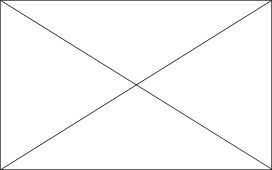
\includegraphics[height=5cm]{Figures/Chapter_1/placeholder} \caption{
			\label{figure_1} One figure using height restriction.}
		\vspace{-0.5cm}
	\end{center}
\end{figure}

\begin{figure}[H] %hbtp
	\begin{center}
		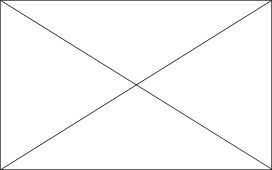
\includegraphics[height=4.5cm]{Figures/Chapter_1/placeholder} 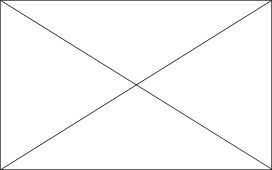
\includegraphics[height=4.5cm]{Figures/Chapter_1/placeholder} \caption{
			\label{figure_2} Two figures using height restriction.}
		\vspace{-0.5cm}
	\end{center}
\end{figure}

\begin{figure}[H] %hbtp
	\begin{center}
		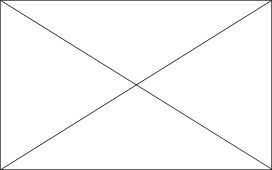
\includegraphics[height=3cm]{Figures/Chapter_1/placeholder} 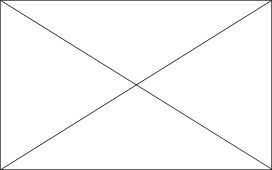
\includegraphics[height=3cm]{Figures/Chapter_1/placeholder} 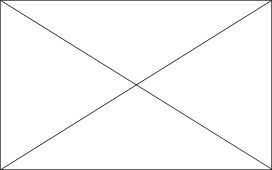
\includegraphics[height=3cm]{Figures/Chapter_1/placeholder} \caption{
			\label{figure_3} Three figures using height restriction.}
		\vspace{-0.5cm}
	\end{center}
\end{figure}

Figures using \textbf{width} restrictions:
\begin{itemize}
	\item One figure (Figure \ref{figure_4})
	\item Two figures (Figure \ref{figure_5})
	\item Three figures (Figure \ref{figure_6})
\end{itemize}

\begin{figure}[H] %hbtp
	\begin{center}
		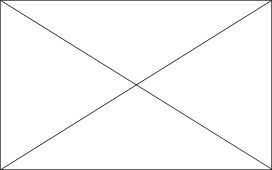
\includegraphics[width=7cm]{Figures/Chapter_1/placeholder} \caption{
			\label{figure_4} One figure using width restriction.}
		\vspace{-0.5cm}
	\end{center}
\end{figure}

\begin{figure}[H] %hbtp
	\begin{center}
		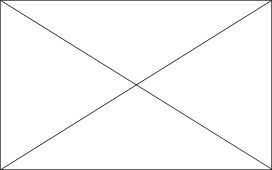
\includegraphics[width=7cm]{Figures/Chapter_1/placeholder} 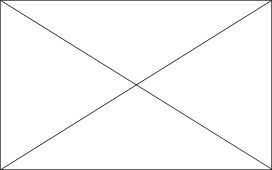
\includegraphics[width=7cm]{Figures/Chapter_1/placeholder} \caption{
			\label{figure_5} Two figures using width restriction.}
		\vspace{-0.5cm}
	\end{center}
\end{figure}

\begin{figure}[H] %hbtp
	\begin{center}
		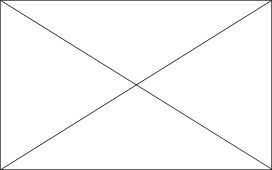
\includegraphics[width=5cm]{Figures/Chapter_1/placeholder} 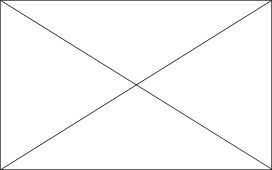
\includegraphics[width=5cm]{Figures/Chapter_1/placeholder} 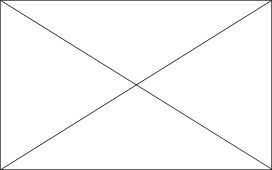
\includegraphics[width=5cm]{Figures/Chapter_1/placeholder} \caption{
			\label{figure_6} Three figures using width restriction.}
		\vspace{-0.5cm}
	\end{center}
\end{figure}

Figures using \textbf{scale} restrictions:
\begin{itemize}
	\item One figure (Figure \ref{figure_7})
	\item Two figures (Figure \ref{figure_8})
	\item Three figures (Figure \ref{figure_9})
\end{itemize}

\begin{figure}[H] %hbtp
	\begin{center}
		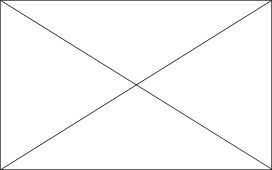
\includegraphics[keepaspectratio=true, scale = 0.75]{Figures/Chapter_1/placeholder} \caption{
			\label{figure_7} One figure using scale restriction.}
		\vspace{-0.5cm}
	\end{center}
\end{figure}

\begin{figure}[H] %hbtp
	\begin{center}
		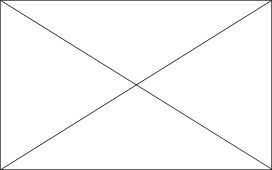
\includegraphics[keepaspectratio=true, scale = 0.6]{Figures/Chapter_1/placeholder} 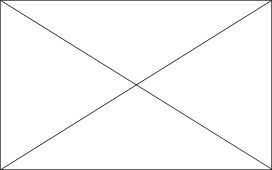
\includegraphics[keepaspectratio=true, scale = 0.6]{Figures/Chapter_1/placeholder} \caption{
			\label{figure_8} Two figures using scale restriction.}
		\vspace{-0.5cm}
	\end{center}
\end{figure}

\begin{figure}[H] %hbtp
	\begin{center}
		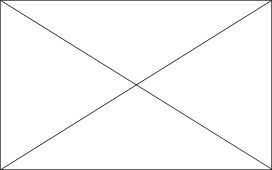
\includegraphics[keepaspectratio=true, scale = 0.5]{Figures/Chapter_1/placeholder} 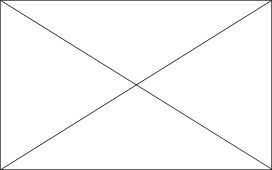
\includegraphics[keepaspectratio=true, scale = 0.5]{Figures/Chapter_1/placeholder} 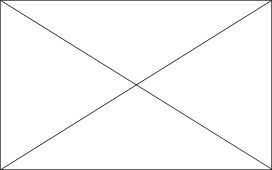
\includegraphics[keepaspectratio=true, scale = 0.5]{Figures/Chapter_1/placeholder} \caption{
			\label{figure_9} Three figures using scale restriction.}
		\vspace{-0.5cm}
	\end{center}
\end{figure}
